\documentclass{cgdrepcn}
\RequirePackage{algpseudocode}
\begin{document}
\title{公司文档管理办法}
\subtitle{(试行)}
\date{}
\author{赵军}
\docattr[docid={CGD-QP-001},
%         relatedid={},
         email={zhaoj@cn.cogenda.com},
%         classification={内部},
         type={质量流程},
         status={试行}]
\maketitle

\begin{abstract}
第一部分为公司文档的管理和排版的要求。第二部分为技术内容和对要求的解释,包括排版软件和排版模板的使用介绍、表格、图片以及代码的排版方式。
\end{abstract}

\begin{revisions}
  0.1 & 2013.12.25 & 赵军 & a draft \\
  0.2 & 2014.01.04 & 沈忱 & translate .tex to .cls \\
  0.3 & 2014.01.10 & 赵军 & refine \\
\end{revisions}

\frontmatter
\tableofcontents
\lstlistoflistings

\mainmatter
\chapter{要求}

为规范公司文档的管理,特制定本办法。目前为试行阶段,欢迎意见和建议。
\section{适用范围}
本管理办法适用于所有权归公司的、密级为“内部”及“公开”的正式文档。包括但不限于:
\begin{itemize}
\item 公司对外的正式报告,比如技术方案、技术总结及操作手册等。
\item 公司对外的书面交流文档。
\item 公司对内的质量流程、开发文档以及有存档价值的过程文档等。
\end{itemize}
不属于此办法管理范围的文档:
\begin{itemize}
\item 密级为“秘密”及以上的文档。
\item 无存档价值的交流文档。
\end{itemize}

\section{排版要求}
公司要求以后的正式文档尽可能用 \LaTeX 排版,并使用公司统一的模板。具体要求和实现方法见本文档后面的部分。

\section{文件存档}

\subsection{应有文件}
每一份文档对应的不是一个文件,而是一个{\bf 目录}。这个目录中应有两个文件:
\begin{enumerate}
\item 最终的 \filename{pdf} 文件。
\item 一个 \filename{zip} 或 \filename{gzip} 包。包中有生成 \filename{pdf} 文件需要的所有 \filename{tex} 文件、图片文件及其他文件如插入代码、原始数据等。
\end{enumerate}
注意事项:
\begin{enumerate}
\item 如果这个文档是用 lyx 软件编辑的,则应在 \filename{zip}/\filename{gzip} 压缩包中包括原始的 \filename{lyx} 文件。
\item 如果文档中的插图是用 LibreOffice 等软件制作的,应在 \filename{zip}/\filename{gzip} 压缩包中包括 \filename{odt}/\filename{odp} 等文件。
\item 如果生成 \filename{pdf} 文件需要特殊的操作步骤,或有其他需要注意的事项,应当在 \filename{README} 文件中加以说明。
\end{enumerate}

\subsection{存档路径}
本办法管理的文档存在公司服务器上,全公司可读。总路径为:\filename{/home/public/document}。以本文档为例,其完整的目录为:\filename{/home/public/document/procedure/CGD-QP-1401/V01/}。其三层路径名:
\begin{itemize}
\item \filename{procedure} 表示本文档的类型为质量流程,
\item \filename{CGD-QP-1401} 为本文档的编号,
\item \filename{V01} 表示其版本。
\end{itemize}
这个路径里面有两个文件,一个 \filename{pdf} 文件,一个原始文件的 \filename{gzip} 包。

\subsection{文档编号规则}
文档编号为 CGD-XX-xxxx,其中 CGD 表示 Cogenda,XX 为字母,表示文档类型。xxxx 为数字,为本文档的顺序号,其中前两个数字为年份,2014 年为 14。编号 XX 对应的类型及其存放路径为:

\begin{ctable}{}{文档类型对应的路径}{lll}
\bf XX & \bf 文档类型 & \bf 存放路径 \\ \hline
TP & 技术方案 & \filename{proposal} \\
TR & 技术总结 & \filename{report} \\
MN & 操作手册 & \filename{manual} \\
QP & 质量流程 & \filename{procedure} \\
MS & 其他文档 & \filename{miscellaneous} \\
\end{ctable}

\subsection{目录名和文件名}
每个文档对应的目录名是文档的完整编号,不可以用其他内容。
文档内的文件名可以自由命名,但只能由英文字母、数字、下划线(\_)或英文句点(.)组成,不可以出现其他字符。

\subsection{入档和查询}
\subsubsection{文件入档}
\begin{enumerate}
\item 如果还没有文档编号,请先跟公司文档管理人员申请编号,填入文档中。
\item 在 helium 下测试一下是否能顺利编译生成 \filename{pdf} 文档。
\item 将所有文件拷给公司文档管理人员。
\end{enumerate}

\subsubsection{文件查询}
目前文档较少,暂时用简单的方式来查询,请用户直接阅读文本文件 \filename{/home/public/document/index}来查询。

\chapter{排版软件及模板的使用方法}
公司在试用了多个排版软件之后,决定选用\LaTeX ,并使用统一的模板。\LaTeX 的工作方式为:用户编辑的文档为纯文本文件,配上用户需要的图片文件(或者原始数据文件),用 \LaTeX 软件处理成为 \filename{ps} 或 \filename{pdf} 文件。如图~\ref{latex} 所示。用户对版式的要求全部写在文本文件中,也就是用户需要了解一些\LaTeX 的排版语法。

\begin{figure}[htbp]\centering
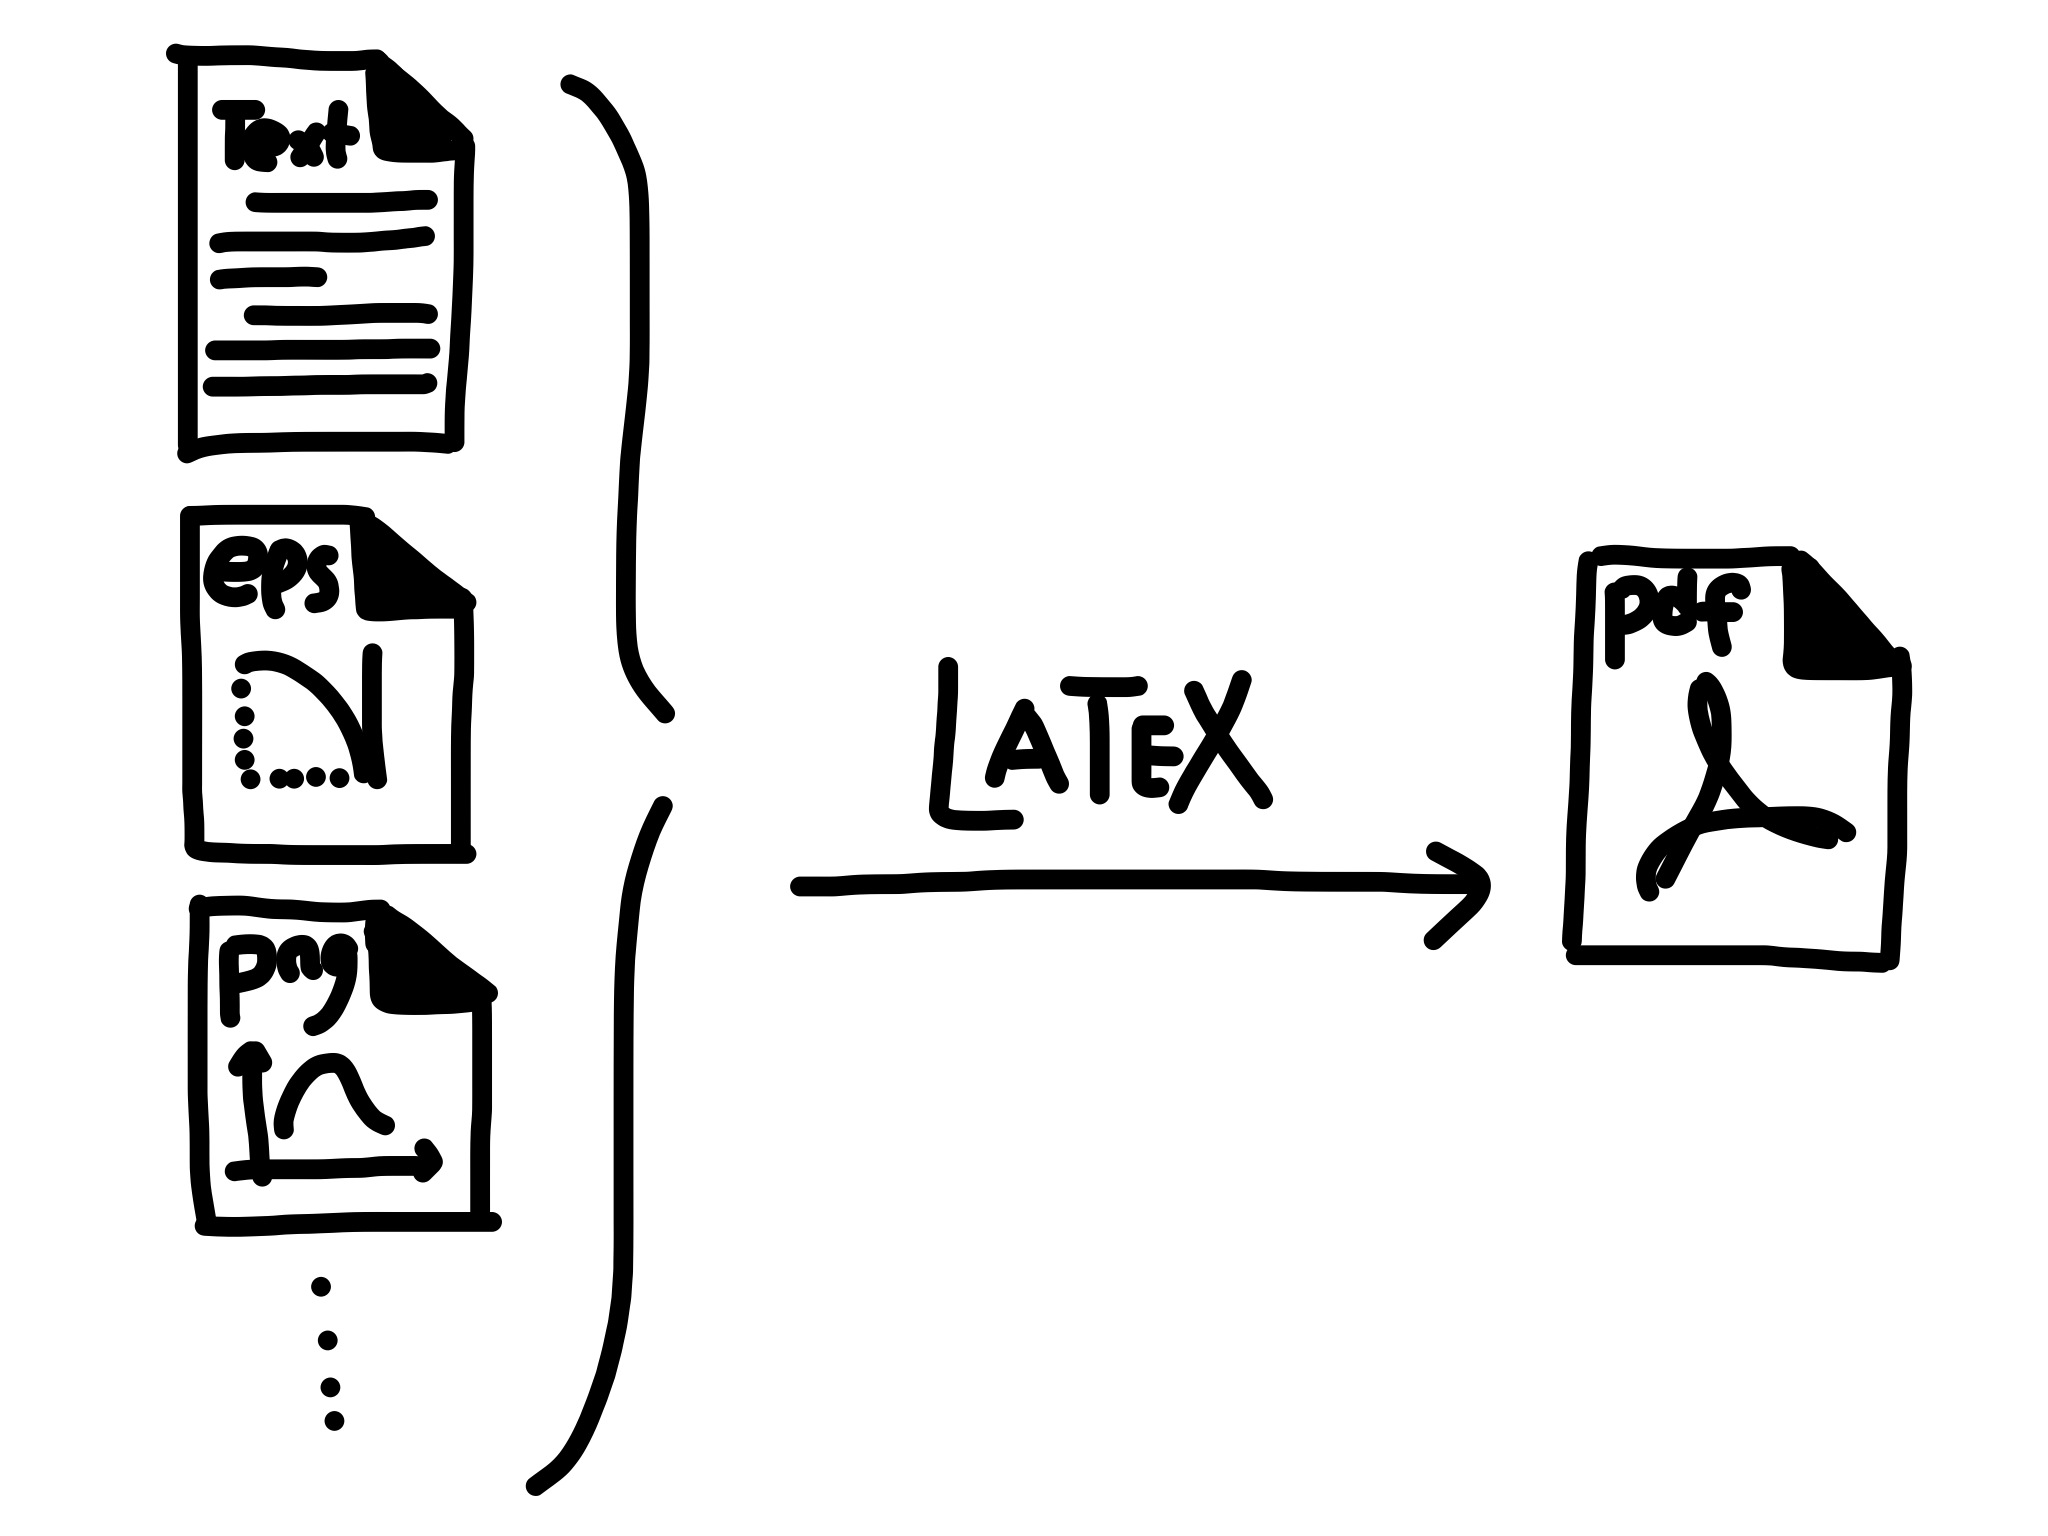
\includegraphics[width=0.45\textwidth]{latex_wm.jpg} 
\caption{\label{latex}\LaTeX 工作方式}
\end{figure}

公司选用\LaTeX 并采用统一的模板,好处为:
\begin{itemize}
\item 统一公司文档的风格。
\item 方便不同的人在不同平台下编辑和修改同一个文档。
\item 对于大型文档,\LaTeX 崩溃的概率小于其他常见排版软件;文本格式的文件损坏的概率也小。
\item \LaTeX 的排版功能非常强大,排出的版面漂亮。
\item \LaTeX 免费。
\end{itemize}
坏处是用户编辑\TeX 文本文档时不够直观。对此公司的建议顺序是:
\begin{enumerate}
\item 使用纯文本编辑器编辑\TeX 文档。(用户可能需要一个\LaTeX 手册\cite{oetiker1995not}。)
\item 用 lyx 编辑。
\item 其他可输出\TeX 文档的软件。要求生成的\TeX 文档适于人工阅读。
\end{enumerate}

\section{软件的安装和使用}
目前我们公司使用的\LaTeX 发行包为 TexLive,你可以直接使用公司 Helium 服务器上的,也可以在自己的电脑上安装一份来用。以下分别介绍。

\subsection{在服务器上使用}
只需要设置使用 TexLive 软件所需的环境。
\begin{lstlisting}[language=sh,caption={在服务器上设置使用 TexLive 的环境}]
# Set the path environment of TexLive 
  source /usr/local/texlive/setenv.sh
# Or to make it permanent, you can simply do:
#    cat /usr/local/texlive/setenv.sh >> $HOME/.bash_profile
# test it
  which xelatex
\end{lstlisting}

\subsection{在自己电脑上安装}
目前我们使用的 TexLive 是个完整的庞大的包,其 \filename{iso} 镜像文件 2.4G,安装后需要 3.5G 的硬盘空间。安装前请在你自己的硬盘上准备充分的空间。
路径为:\filename{/home/public/software/tex/texlive2013/},文件为\filename{texlive2013-*.iso}。对于 Linux 系统,可能需要几个字体文件。字体文件为 \filename{win\_fonts.tar.gz }和\filename{STIXv1.1.0.zip}。

假设你准备把字体安装在 \filename{/usr/share/fonts/TTF/}。安装方法为:
\begin{lstlisting}[language=sh,caption={安装字体}]
# copy the font files
  tar -xzvf win_fonts.tar.gz && sudo cp -r win_fonts /usr/share/fonts/TTF/
# activate the fonts
  sudo fc-cache -fv
\end{lstlisting}

假设你准备把 TexLive 安装在 \filename{/usr/local/tex} 。安装方法为:
\begin{lstlisting}[language=sh,caption={安装 TexLive}]
# mount the iso file
  sudo mount -o loop texlive2013-20130530.iso /mnt/dvd  && cd /mnt/dvd
# install it
  export TEXLIVE_INSTALL_PREFIX=/usr/local/tex
  perl install-tl
# then follow the instructions to set the path environment
  export PATH=/usr/local/texlive/2013/bin/x86_64-linux:$PATH
\end{lstlisting}

对于 Windows 用户,以上镜像文件也支持 Windows。请阅读镜像文件里的说明文件。

\subsection{Lyx}
Lyx 是一个直观的编辑\TeX 文件的编辑器。不需要 lyx 的人可以不用理会下文中提到lyx的段落。Helium 服务器上已经安装了 lyx,你可以直接使用,也可以在自己电脑上安装。

\section{模板的安装和使用}
\subsection{服务器上使用 texlive}
如果用户不需要 lyx,公司模板已经安装。用户只需要拷贝一个例子,照这个例子填入自己的内容便可。例子在下文中的模板文件中,解压后直接使用,不需要安装。

如果需要使用 lyx,则用户需要在自己的路径下安装模板。在安装模板之前,需要先启动 lyx 一次以生成\filename{\$HOME/.lyx}。模板的路径:\filename{/home/public/document/template/cgdrep.tar.gz}。安装方法:
\begin{lstlisting}[language=sh,caption={安装模板}]
# Unpack the template
  tar xf /home/public/document/template/cgdrep.tar.gz
  cd cgdrep
# Install the template files
  ./install.sh
\end{lstlisting}

对于 lyx 用户,安装模板之后,启动 lyx 并点击\guimenu{Tools>{Reconfigure}},然后重新启动 lyx。

\subsection{用户在自己机上安装模板}
不论是否需要 lyx,都需要安装模板。安装方法同上一小节。

\subsection{模板的使用}
以上安装中不报错的话,可以使用 \LaTeX 模板里面的示例了:
\begin{lstlisting}[language=sh,caption={模板示例}]
# test the LaTeX example
  cd example/latex
  make
# There should be several new files and one of them is main.pdf
  evince main.pdf &
\end{lstlisting}

示例中的\command{make}命令编译了四遍,这可能需要些时间。用户如果想快速看到结果的话,可以只编译一遍,命令为\command{xelatex main}。这样得到的\filename{pdf} 结果并不完整:可能没有包含参考文献,交叉引用可能不正确。要得到最后的正式 \filename{pdf}文件,还是需要\command{make} 一下的。


\chapter{模板的格式要求}
我们暂定了表格、图片、代码和其他一些对象的格式要求,并写了一些宏放在模板里。目前这些格式要求并不是最终版,欢迎提出意见。

一般,每一个表格(图片、代码)都当有一对\filename{Caption} 和\filename{Label}。\filename{Caption} 是这个表格(图片、代码)的名字,其字号比正文小半号。\filename{Label} 是引用它时用的标识,\filename{Label} 本身的内容并不出现在排版后的\filename{pdf}页面上。以下分别讲如何实现表格、图片和代码格式的实现方法。

\section{表格}
用户没有特别需要的话,我们希望表格都采用三线表,首行为其\filename{header},用黑体。字号比正文小半号,位置居中。如表~\ref{triline}:
\begin{ctable}{triline}{三线表}{llll}
 版本 & 日期       & 负责人       & 备注 \\ \hline 
 1.0  & 2013.12.24 & 沈忱、纪冬梅 & 初稿 \\
 1.1  & 2013.12.25 & 赵军         & 二稿 \\
\end{ctable}

实现这样的表及其浮动位置,可以用公司自己制作的宏 \filename{ctable},其语法为:
\begin{lstlisting}[language={[LaTeX]TeX},caption={ctable 语法}]
\begin{ctable}{Label}{Caption}{Alignments}
 第一行(header)  \\ \hline 
 第二行 \\
.....
\end{ctable}\end{lstlisting}

其中\filename{Alignments}是列对齐方式,四列左对齐为\filename{\{llll\}}。则表~\ref{triline} 的完整语法为:
\begin{lstlisting}[language={[LaTeX]TeX},caption={ctable 示例}]
\begin{ctable}{triline}{三线表}{llll}
 版本 & 日期       & 负责人       & 备注 \\ \hline 
 1.0  & 2013.12.24 & 沈忱、纪冬梅 & 初稿 \\
 1.1  & 2013.12.25 & 赵军         & 二稿 \\
\end{ctable}
\end{lstlisting}

如果你不想局限于 \filename{ctable} 的功能,也可以用一般的 \LaTeX 表格语法(模板包含了 \filename{tabu} 宏包),表~\ref{triline} 的一般\LaTeX 语法为:
\begin{lstlisting}[language={[LaTeX]TeX},caption={三线表的一般\LaTeX 语法示例}]
\begin{table}[htbp]\caption{\label{triline} 三线表}
\centering\small\begin{tabu}{llll}\thickhline\rowfont{\bfseries}
 版本  & 日期       & 负责人      & 备注 \\ \hline
 1.0  & 2013.12.24 & 沈忱、纪冬梅 & 初稿 \\
 1.1  & 2013.12.25 & 赵军         & 二稿 \\
\thickhline\end{tabu}\end{table}
\end{lstlisting}

\section{图片}
插入图片的语法简单,这里没有设置自己的宏,而是用的是普通语法:
\begin{lstlisting}[language={[LaTeX]TeX},caption={插入图片语法示例}]
\begin{figure}[htbp]\centering
\includegraphics[width=0.5\textwidth]{file.jpg} 
\caption{\label{Label}Caption}
\end{figure}\end{lstlisting}
对于图片的大小控制,当用户没有特别需求的时候,建议采用\filename{textwidth}的倍数方式。

\section{代码}
这里先给出一段文档中插入 Pascal 代码的样子:
\begin{lstlisting}[language=Pascal,caption={Pascal 代码示例},label=PascalExample]
for i:=maxint to 0 do
begin
{ do nothing }
end;
Write(’Case insensitive ’);
Write(’Pascal keywords.’);
\end{lstlisting}

插入代码的 \LaTeX 语法为:
\begin{lstlisting}[language={[LaTeX]TeX},caption={插入代码的语法}]
\begin{lstlisting}[language=Language,caption={Caption},label=Label]
.......
 (代码内容)
.......
\end{lstlisting }\end{lstlisting}

其中\filename{Languge}为这一段代码的语言。支持的语言包括 ABAP、ACSL、Ada、Algol、Ant、Assembler、Awk、bash、Basic、C、C++、Caml、Clean、Cobol、Comal、csh、Delphi、Eiffel、Elan、erlang、Euphoria、Fortran、GCL、Gnuplot、Haskell、HTML、IDL、inform、Java、JVMIS、ksh、Lisp、Logo、make、Mathematica、Matlab、Mercury、MetaPost、Miranda、Mizar、ML、Modelica、Modula-2、MuPAD、NASTRAN、Oberon-2、OCL、Octave、Oz、Pascal、Perl、PHP、PL/I、Plasm、POV、Prolog、Promela、Python、R、Reduce、Rexx、RSL、Ruby、S、SAS、Scilab、sh、SHELXL、Simula、SQL、tcl、TeX、VBScript、Verilog、VHDL、VRML、XML、XSLT。更多信息请搜索关键词 lstlisting。代码~\ref{PascalExample} 的引用方法为:
\begin{lstlisting}[language={[LaTeX]TeX},caption={插入代码示例}]
\begin{lstlisting}[language=Pascal,caption={Pascal 示例代码},label=PascalExample]
for i:=maxint to 0 do
begin
{ do nothing }
end;
Write(’Case insensitive ’);
Write(’Pascal keywords.’);
\end{lstlisting }
\end{lstlisting}

目前暂定代码的文字大小为 \filename{\textbackslash footnotesize}。如果用户需要调整,可以在引用前修改字体,比如大半号为\filename{\textbackslash small},其语法为:
\begin{lstlisting}[language={[LaTeX]TeX}]
\lstset{basicstyle=\small\ttfamily}
\end{lstlisting}
这个命令将作用于后面所有的代码。如果这并不是用户想要的,则需要修改回来:
\begin{lstlisting}[language={[LaTeX]TeX}]
\lstset{basicstyle=\footnotesize\ttfamily}
\end{lstlisting}
同理,用户也可以一次设定语言:
\begin{lstlisting}[language={[LaTeX]TeX}]
\lstset{languge=Language}
\end{lstlisting}
则后面每次插入代码时候就不用加入\filename{language=Languge}这一句了。更详细的用法请搜索关键词 lstlisting。

如果代码比较长,在某个原始代码文件里,可以用如下语法,将整个文件的代码引入:
\begin{lstlisting}[language={[LaTeX]TeX},caption={引入代码文件示例}]
\lstinputlisting[language=Language,label=Label,caption={Caption}]{Filename}
\end{lstlisting}

下面给出 C、Python 和 Bash 代码示例,欢迎提出排版意见。

\begin{lstlisting}[language=C,caption={C 代码示例},label=cLabel]
#include <stdio.h>
#define N 10
/* Block
 * comment */
 
int main()
{
    int i;
 
    // Line comment.
    puts("Hello world!");
 
    for (i = 0; i < N; i++)
    {
        puts("LaTeX is also great for programmers!");
    }
 
    return 0;
}
\end{lstlisting}

\begin{lstlisting}[language=python,caption={Python 代码示例},label=Python]
class BankAccount(object):
    def __init__(self, initial_balance=0):
        self.balance = initial_balance
    def deposit(self, amount):
        self.balance += amount
    def withdraw(self, amount):
        self.balance -= amount
    def overdrawn(self):
        return self.balance < 0
my_account = BankAccount(15)
my_account.withdraw(5)
print my_account.balance
import unittest
def median(pool):
    copy = sorted(pool)
    size = len(copy)
    if size % 2 == 1:
        return copy[(size - 1) / 2]
    else:
        return (copy[size/2 - 1] + copy[size/2]) / 2
class TestMedian(unittest.TestCase):
    def testMedian(self):
        self.failUnlessEqual(median([2, 9, 9, 7, 9, 2, 4, 5, 8]), 7)
if __name__ == '__main__':
    unittest.main()
\end{lstlisting}

\lstinputlisting[language=bash,label=bash.sh, caption={bash 代码示例}]{bash1.sh}

\section{其他格式要求}
\subsection{几个字体宏}
有几个特别对象,要在文档里用特别的字体来,我们定义了几个字体的宏,如表~\ref{special} 所列。文档中用到这样的对象时,请采用表中的字体宏。

\begin{ctable}{special}{几类特别对象}{lll} 
对象 & 语法示例 & 效果示例 \\ \hline
文件名 & \textbackslash filename\{directory/file.name\} & \filename{directory/file.name} \\
命令名 & \textbackslash command\{xelatex main\} & \command{xelatex main} \\
参数名 & \textbackslash parameter\{Energy\} & \parameter{Energy} \\
用户输入 & \textbackslash userinput\{runApp\} & \userinput{runApp} \\
图形界面菜单 & \textbackslash guimenu\{File > Open\} & \guimenu{File>Open} \\
\end{ctable}

\subsection{Item 列表}
对于三个 item 列表(itemize、enumerate和description),我们都改了间距。如果用户想在每个 item 里放一段落,于是想保留段落间距的话,可以用新的环境变量 paraitem。语法为:
\begin{lstlisting}[language={[LaTeX]TeX},caption={保留段落间距的环境变量}]
\begin{paraitem}
\item 第一段。
\item 第二段。
.....
\end{paraitem}
\end{lstlisting}


\chapter{对某些对象的排版要求}
\lstset{language={[LaTeX]TeX}}
本章介绍的是关于几个常用对象的排版要求。这些要求的效果属于常见的排版效果,于是公司模板中不需要自定义的宏包,只在本章做些要求或建议。为帮助理解这些要求和建议,本章会对一些基本概念做简单的解释,而这些解释不足以向新手介绍清楚对象的用法。

\section{用户自己增加宏包}
如果用户需要增加新的宏包,可以在 preamble 区(\filename{\textbackslash documentclass} 语句之后,\filename{\textbackslash begin\{document\}} 语句之前)加入语句\filename{\textbackslash RequirePackage\{Package\}}。不建议用\filename{\textbackslash usepackage}。

\section{交叉引用和参考文献}
\LaTeX 排版的一个优点是交叉引用的逻辑清晰而严谨,以下做一个简单的介绍。

\subsection{交叉引用}
所有有\filename{Label} 的表格、图片、代码、公式和章节都可以被引用,语法为\filename{\textbackslash ref\{Label\}}。举例:如果想实现“如表~\ref{triline} 所示”字样,\LaTeX 语法为
\footnotesize\begin{verbatim}
如表~\ref{triline} 所示
\end{verbatim}
\normalsize
中间的波浪线的功能是实现“表”字与编号 \ref{triline} 之间的留空。这个留空不用普通的空格来实现,是为了避免在这里换行。

如果想提到某一\filename{Label}对象所在的页码,语法为\filename{\textbackslash pageref\{Label\}}。如果想给某些章节加\filename{Label},方法是在章节名如 \filename{\textbackslash chapter\{Chapter\}}后加一句\filename{\textbackslash label\{Label\}}。\filename{Label} 可能会非常多,作者自己会记不请。对此可参考的建议有:
\begin{itemize}
\item 不需要引用的就不用给\filename{Label},等到需要的时候再给也不迟。
\item 分类取名,比如表格都用\filename{tab:}开头,图片都用\filename{fig:}开头。
\item 用比较清晰的英文简称作为\filename{Label}。
\end{itemize}

\subsection{参考文献及引用}
建议参考文献用\command{bibtex} 来编译。参考文献集中在文件 \filename{main.bib}中,文献格式示例:
\begin{lstlisting}[caption={参考文献格式示例}]
@article{katz1979history,
  title={The History of Stokes's Theorem},
  author={Victor J. Katz},
  journal={Mathematics Magazine},
  volume={52},
  pages={146-156},
  year={1979},
}
\end{lstlisting}
Label 在其中第一行。

这篇文献的引用方法为:
\begin{lstlisting}
\cite\{katz1979history\}
\end{lstlisting}

\section{数学环境}
\LaTeX 是数学系的至爱,因为其数学公式排版漂亮。\LaTeX 有三种数学环境:
\begin{enumerate}
\item math:行内数学环境,像在正文行内出现 $E=mc^2$ 这样。
\item displaymath:独立占行,不参与公式编号,无\filename{Label}。
\item equation:独立占行,参与公式编号,可以设\filename{Label}来引用。
\end{enumerate}

我们要求所有的数学内容都用数学环境,包括物理量。比如提到深度变量的时候用 $d$ 而不是 d,前者变用了 math 环境。排出漂亮的公式需要不少数学语法,可以准备网页版的参考手册,也可以考虑 lyx 或其他软件来生成。

\begin{paraitem}
\item math 环境的语法为两端用\textbackslash(和\textbackslash)括起来(或者用\$括起来)。例如质能方程的语法为\textbackslash(E=mc\^{}2\textbackslash),也可以是\$E=mc\^{}2\$。

\item display 环境的语法是两端用\textbackslash[和\textbackslash]括起来。(也可以用 \$\$ 括,但据介绍可能会与其他宏包冲突,不推荐。)举例:\[\int_0^\infty \mathrm{e}^{-x}\,\mathrm{d}x\]
其语法为:
\begin{lstlisting}
\[ \int_0^\infty \mathrm{e}^{-x}\,\mathrm{d}x \]
\end{lstlisting}

\item equation 环境来表达同一个积分式,效果为:
\begin{equation}\label{eq:integral}
\int_0^\infty \mathrm{e}^{-x}\,\mathrm{d}x
\end{equation}
式~\ref{eq:integral} 的语法为:
\begin{lstlisting}
\begin{equation}\label{eq:integral}
\int_0^\infty \mathrm{e}^{-x}\,\mathrm{d}x
\end{equation}
\end{lstlisting}
\end{paraitem}

需要注意的是,在数学模式中,一般的字母会被解释为变量,于是变成了斜体,当你不需要斜体的时候,就要作特别声明,如\filename{\textbackslash mathrm}。也有宏包做其他的定义方式,$\diff x$ 中的 $\diff$ 可以用\filename{\textbackslash diff};$r=\unit{2.5cm}$ 中的 $\unit{2.5cm}$ 可以用\filename{\textbackslash unit\{2.5cm\}}。


\section{算法}
有些宏包可以帮助\LaTeX 排版算法(伪代码)。这里举一个例子:
\begin{algorithmic}
\If {$i\geq maxval$}
    \State $i\gets 0$
\Else
    \If {$i+k\leq maxval$}
        \State $i\gets i+k$
    \EndIf
\EndIf
\end{algorithmic}

这个例子的代码为(用了\filename{algpseudocode} 宏包):
\begin{lstlisting}
\begin{algorithmic}
\If {$i\geq maxval$}
    \State $i\gets 0$
\Else
    \If {$i+k\leq maxval$}
        \State $i\gets i+k$
    \EndIf
\EndIf
\end{algorithmic}
\end{lstlisting}


\appendix

\bibliographystyle{ieeetr}
\bibliography{main}

\backmatter

\end{document}

